% ----------------------------------------------------------
\chapter{Resultados e Discussão}\label{cap:resultados}
% ----------------------------------------------------------

Este capítulo apresenta os resultados na ordem do processamento: calibração e medição, segmentação, classificação da maturação, detecção de defeitos e desempenho do sistema completo no conjunto de teste. Ao final, os resultados são comparados com os critérios de aceitação e as limitações do estudo são discutidas.

% ----------------------------------------------------------
\section{Calibração e Medição de Tamanho}
% ----------------------------------------------------------

A calibração de escala (\autoref{fig:escala}) apresentou resíduo máximo de 0,46 mm, na célula inferior direita, dentro do limite de 0,5 mm; por ser calculado com o próprio tabuleiro, esse resíduo mede a consistência da calibração, e não a exatidão em outros objetos, avaliada a seguir com a moeda. A escala variou 3,6\% entre a maior e a menor célula, e cerca de 2,4\% entre as médias da linha superior e da inferior. Uma variação gradual e aproximadamente linear desse tipo é típico de uma câmera ligeiramente inclinada em relação ao plano, e não de distorção da lente, que seria simétrica em torno do centro da imagem.

A \autoref{tab:moeda} resume as 64 medições da moeda de 27,00 mm distribuídas pelas nove células. A correção por região reduziu o desvio padrão das medidas quase pela metade (de 0,32 para 0,17 mm), isto é, tornou a medida menos dependente da posição do objeto na imagem, e o erro médio absoluto de 0,45 mm ficou abaixo do limite de 1 mm. Em uma mesma posição, sem reposicionar a moeda, o desvio padrão foi de 0,01 a 0,03 mm; esse valor mede o ruído da câmera e da segmentação, e não a repetibilidade de posicionamento. Como as medições repetidas na mesma posição não são independentes, a estatística por posição (uma média para cada uma das dez primeiras posições) também foi calculada e deu resultado semelhante: erro médio absoluto de 0,53 mm com correção.

\begin{table}[htb]
	\ABNTEXfontereduzida
	\centering
	\caption{\label{tab:moeda}Erro na medição do diâmetro de uma moeda de 27,00 mm (64 medições em todas as células).}
	\begin{tabular}{lccccc}
		\toprule
		Escala & Erro médio & Desvio padrão & Erro médio absoluto & RMSE & Faixa do erro \\
		 & (mm) & (mm) & (mm) & (mm) & (mm) \\
		\midrule
		Única (média) & $-0{,}48$ & 0,32 & 0,49 & 0,57 & $-1{,}16$ a $+0{,}11$ \\
		Por região & $-0{,}45$ & 0,17 & 0,45 & 0,48 & $-0{,}82$ a $-0{,}21$ \\
		\bottomrule
	\end{tabular}
	\fonte{Elaborado pelo autor (2026).}
\end{table}

A correção por região, porém, não removeu o viés: todas as medições com correção ficaram abaixo do valor real, em média 0,45 mm. As causas foram investigadas. A segmentação não corta a borda da moeda: no perfil de brilho radial, o contorno segmentado ficou 0,7 pixel por fora da borda, o que aumentaria a medida. A espessura da moeda, cerca de 2 mm mais próxima da câmera, também aumentaria a medida (cerca de 0,7\%). O tamanho dos quadrados impressos do tabuleiro foi conferido. A explicação mais provável é que o tabuleiro e a moeda não estivessem exatamente no mesmo plano (por exemplo, por diferença de altura ou inclinação do papel sobre o tecido), o que é coerente com a limitação do modelo \textit{pinhole} discutida no \autoref{cap:revisao}. Essa hipótese não foi testada. Um fator de correção calculado com essas mesmas medições não foi aplicado, pois o sistema seria validado com os dados usados para ajustá-lo.

Nos tomates, a medição não pôde ser validada, pois o diâmetro com paquímetro não foi registrado nos rótulos. No conjunto de teste, os diâmetros equivalentes medidos variaram de 18,9 a 32,2 mm (mediana de 26,2 mm) e a circularidade de 0,51 a 0,86 (mediana de 0,79). A circularidade ficou bem abaixo da da moeda (0,91 a 0,92). O alongamento explica só parte disso: uma elipse com razão de 1,5 entre os eixos ainda tem circularidade de cerca de 0,94, e o tomate 11, com razão de 1,3, teve circularidade de 0,51. Os valores baixos refletem principalmente irregularidades do contorno, como defeitos, cálice e ruído da segmentação, que aumentam o perímetro.

% ----------------------------------------------------------
\section{Segmentação}
% ----------------------------------------------------------

A segmentação encontrou um único objeto em cada uma das 22 fotos do conjunto de teste, sem objetos espúrios. No tomate 16, porém, o objeto segmentado tem 47,9 mm de comprimento por 22,0 mm de largura, com um estreitamento no meio, o que sugere dois frutos encostados segmentados como um só; se for o caso, a segmentação acertou 21 das 22 fotos. No conjunto de defeitos, apenas as 2 fotos de um tomate que não estava inteiramente dentro da região de interesse foram rejeitadas, como previsto. O uso do maior canal de cor, em vez do nível de cinza, foi decisivo durante o desenvolvimento: com o nível de cinza, um tomate vermelho-escuro ficava abaixo do contraste mínimo, e a presença de um objeto branco na região deslocava o limiar de Otsu a ponto de perder os tomates.

As imagens da bancada, contudo, são escuras (\autoref{fig:testeexemplos}): mesmo após o balanço de branco, os frutos aparecem com pouco brilho sobre o fundo preto, o que se deve à iluminação fraca já indicada pelos ganhos elevados na calibração de branco.

% ----------------------------------------------------------
\section{Classificação da Maturação}
% ----------------------------------------------------------

\subsection{Validação da LUT}

No nível do pixel, segundo o registro de execução do programa, a MLP acertou 99,7\% dos pixels dos tomates reservados para validação. Esse número, entretanto, é pouco informativo: os rótulos dos pixels vêm dos grupos do \textit{k-means}, que foram calculados com todas as fotos, inclusive as de validação, e os tomates de validação não incluíam nenhum imaturo, pois havia apenas dois tomates imaturos no conjunto de cor.

Aplicada às 50 fotos aproveitáveis do conjunto de cor, a regra de maturação acertou 62\% tanto nos tomates de validação (5 de 8 fotos) quanto nos de treino (26 de 42 fotos). Todos os erros foram de tomates rotulados como intermediários e classificados como maduros: 16 das 19 fotos de intermediários usadas no treino tinham mais de 60\% da superfície classificada como vermelha. A causa principal está nos próprios grupos de cor. O grupo nomeado rosado tem praticamente a mesma matiz dos grupos vermelhos (ângulo de cerca de 36$^\circ$ no plano a*b*, contra 34$^\circ$ a 37$^\circ$) e difere deles apenas por ser mais claro; todos os grupos têm luminosidade baixa (L* entre 16 e 31). Assim, a separação entre rosado e vermelho depende do brilho, e não da cor, e com a iluminação fraca da bancada a maior parte da superfície de um fruto rosado é classificada como vermelha. Contribui também a subjetividade do rótulo: a fronteira entre os estádios rosado e vermelho claro do USDA é estreita, e o rótulo foi atribuído visualmente.

\subsection{Conjunto de teste}

No conjunto de teste, a maturação foi classificada corretamente em 19 dos 22 tomates (86,4\%; IC 95\%: 66,7\% a 95,3\%), conforme a \autoref{tab:maturacao}. Esse valor, porém, é dominado pelos tomates maduros, que formam 17 dos 22 frutos e foram todos acertados. Nas classes minoritárias, o desempenho foi baixo: 2 de 4 intermediários e nenhum dos imaturos (havia apenas um). Um dos intermediários acertados (tomate 14) teve 59,9\% da superfície vermelha, praticamente sobre o limite de 60\%. Os dois intermediários errados tinham 91\% da superfície classificada como vermelha, repetindo o padrão observado no conjunto de cor. O tomate imaturo (\autoref{fig:testeexemplos}d), esverdeado com regiões alaranjadas, teve 83\% da superfície classificada como colorida (25\% como vermelha), muito acima do limite de 10\% para imaturo, e foi classificado como intermediário: os grupos nomeados como verde reúnem apenas 6\% dos pixels de treino, e os tons verde-amarelados escuros desse fruto foram atribuídos a classes coloridas. A média das taxas de acerto por classe é de apenas 50\%, o que mostra que a acurácia global superestima a capacidade da LUT de distinguir os estádios.

\begin{table}[htb]
	\centering
	\caption{\label{tab:maturacao}Matriz de confusão da maturação no conjunto de teste (22 tomates).}
	\begin{tabular}{lccc}
		\toprule
		Real $\backslash$ LUT & Imaturo & Intermediário & Maduro \\
		\midrule
		Imaturo & 0 & 1 & 0 \\
		Intermediário & 0 & 2 & 2 \\
		Maduro & 0 & 0 & 17 \\
		\bottomrule
	\end{tabular}
	\fonte{Elaborado pelo autor (2026).}
\end{table}

Assim, o critério de 90\% de acurácia na maturação não foi atingido, e a LUT, na forma atual, separa bem os frutos maduros, mas não distingue com confiabilidade os estádios intermediários. As causas identificadas são os grupos de cor que separam rosado e vermelho pelo brilho, a pouca quantidade de tomates imaturos e intermediários no conjunto de cor, a iluminação fraca, que exige ganho alto no canal vermelho, e a subjetividade dos rótulos.

% ----------------------------------------------------------
\section{Detecção de Defeitos}
% ----------------------------------------------------------

\subsection{Validação cruzada}

A \autoref{tab:cnncv} apresenta a validação cruzada da CNN em 5 partes, com divisão por tomate e métricas calculadas por foto. A acurácia balanceada média foi de 93,6\% $\pm$ 1,9\% (desvio padrão populacional entre as partes), com sensibilidade de 95,0\% e especificidade de 92,1\%. Somando as partes, 113 das 119 fotos de tomates com defeito foram detectadas, e 11 das 140 fotos de tomates sadios foram classificadas como defeituosas.

\begin{table}[htb]
	\ABNTEXfontereduzida
	\centering
	\caption{\label{tab:cnncv}Validação cruzada da CNN em 5 partes, com divisão por tomate (métricas por foto).}
	\begin{tabular}{cccccc}
		\toprule
		Parte & Melhor época & Acurácia & Acur. balanceada & Sensibilidade & Especificidade \\
		\midrule
		1 & 24 & 90,4\% & 90,5\% & 91,7\% & 89,3\% \\
		2 & 22 & 96,2\% & 96,1\% & 95,8\% & 96,4\% \\
		3 & 28 & 94,2\% & 94,3\% & 95,8\% & 92,9\% \\
		4 & 8 & 94,2\% & 94,3\% & 95,8\% & 92,9\% \\
		5 & 30 & 92,2\% & 92,5\% & 95,7\% & 89,3\% \\
		\midrule
		Média & -- & 93,4\% & 93,6\% & 95,0\% & 92,1\% \\
		Desvio padrão & -- & 2,0\% & 1,9\% & 1,7\% & 2,7\% \\
		\bottomrule
	\end{tabular}
	\fonte{Elaborado pelo autor (2026).}
\end{table}

As curvas de aprendizado (\autoref{fig:curvas}) mostram a perda de treino diminuindo de forma contínua, enquanto a perda de validação oscila bastante de uma época para a outra, comportamento esperado com cerca de 50 fotos de validação por parte, em que poucas imagens mudam a métrica. A melhor época variou de 8 a 30 entre as partes, e o modelo final foi treinado por 24 épocas (a mediana). Na parte 5, a melhor época coincidiu com o limite de 30, o que indica que um limite maior poderia ter sido testado. Em uma versão preliminar, treinada com apenas 28 tomates, a validação cruzada havia resultado em 94,5\% $\pm$ 3,7\%.

A média da validação cruzada, porém, é dominada pela primeira sessão de captura, em que todos os sadios foram fotografados antes dos defeituosos e que responde por 176 das 259 fotos. Separando os erros por sessão, a primeira teve especificidade de 96,1\% (98 de 102 fotos de sadios) e sensibilidade de 94,6\% (70 de 74), enquanto as sessões seguintes, com classes intercaladas, tiveram especificidade de apenas 81,6\% (31 de 38) e sensibilidade de 95,6\% (43 de 45), com acurácia balanceada de cerca de 88,6\%. Não é possível afirmar que a rede tenha aprendido características da sessão, e não do fruto, mas a diferença é compatível com isso, e o fundo não mascarado do recorte tornaria esse aprendizado possível.

\begin{figure}[htb]
	\caption{\label{fig:curvas}Curvas de aprendizado de duas partes da validação cruzada: perda de treino (azul) e de validação (vermelho), normalizadas pela perda máxima, e acurácia balanceada de validação (verde). A linha vertical marca a melhor época.}
	\centering
	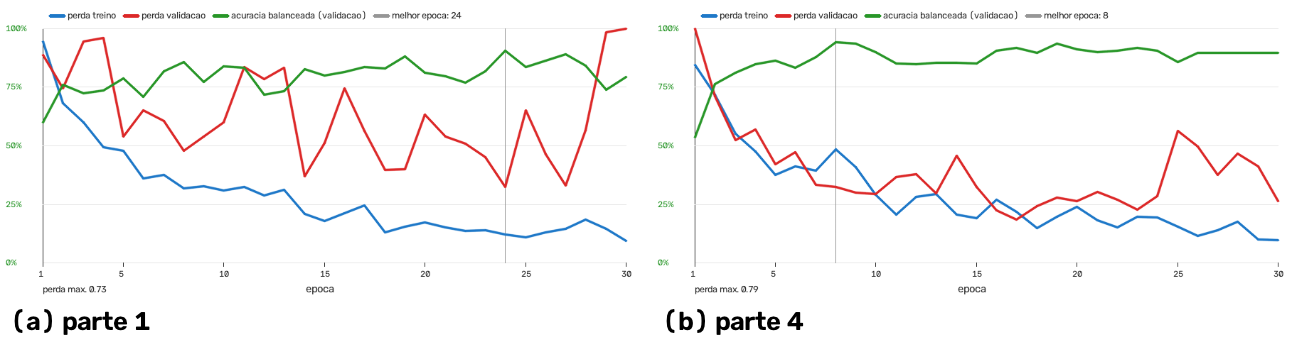
\includegraphics[width=\textwidth]{images/curvas_cnn.png}
	\fonte{Elaborado pelo autor (2026).}
\end{figure}

O modelo exportado em ONNX e executado pelo OpenCV reproduziu as probabilidades do PyTorch com diferença máxima de 0,0013 (registrada no arquivo de execução do treino), confirmando que a interface usa o mesmo modelo avaliado.

\subsection{Conjunto de teste}

No conjunto de teste (\autoref{tab:cnnteste}), a CNN classificou corretamente 19 dos 22 tomates (86,4\%), com sensibilidade de 84,6\% (11 de 13 defeituosos detectados) e especificidade de 88,9\% (8 de 9 sadios aceitos), precisão de 91,7\% e F1 de 0,88. Por reamostragem (\textit{bootstrap}, 20.000 amostras) dos 22 tomates, o intervalo de 95\% do F1 vai de 0,71 a 1,00, e 33\% das reamostras ficam abaixo de 0,85. O resultado de cada tomate está no \autoref{ap:teste}.

\begin{table}[htb]
	\centering
	\caption{\label{tab:cnnteste}Desempenho da CNN no conjunto de teste (22 tomates, uma foto cada), com intervalos de confiança de Wilson (95\%).}
	\begin{tabular}{lcc}
		\toprule
		Métrica & Valor & IC 95\% \\
		\midrule
		Acurácia & 86,4\% (19/22) & 66,7\% a 95,3\% \\
		Sensibilidade & 84,6\% (11/13) & 57,8\% a 95,7\% \\
		Especificidade & 88,9\% (8/9) & 56,5\% a 98,0\% \\
		Acurácia balanceada & 86,8\% & -- \\
		F1 (classe com defeito) & 0,88 & 0,71 a 1,00 (\textit{bootstrap}) \\
		\bottomrule
	\end{tabular}
	\fonte{Elaborado pelo autor (2026).}
\end{table}

Os três erros estão ilustrados na \autoref{fig:testeexemplos}. Os dois defeitos não detectados foram uma mancha (tomate 7, probabilidade de defeito de 0,03) e um dano mecânico (tomate 22, probabilidade de 0,19), defeitos pequenos e de baixo contraste nas imagens escuras da bancada. O tomate sadio descartado (tomate 16, probabilidade de 0,72) é o objeto alongado discutido na seção de segmentação, possivelmente dois frutos encostados. Em qualquer caso, é uma imagem atípica em relação às de treino, e o erro é possivelmente relacionado à dificuldade das redes com entradas afastadas da distribuição de treino \cite{nguyen2015,hendrycks2017}.
% FIXME (autor): conferir na foto original se o tomate 16 é um único fruto alongado ou dois frutos encostados.

\begin{figure}[htb]
	\caption{\label{fig:testeexemplos}Exemplos do conjunto de teste, como exibidos pela IHM: o contorno tem a cor do destino decidido pelo sistema.}
	\centering
	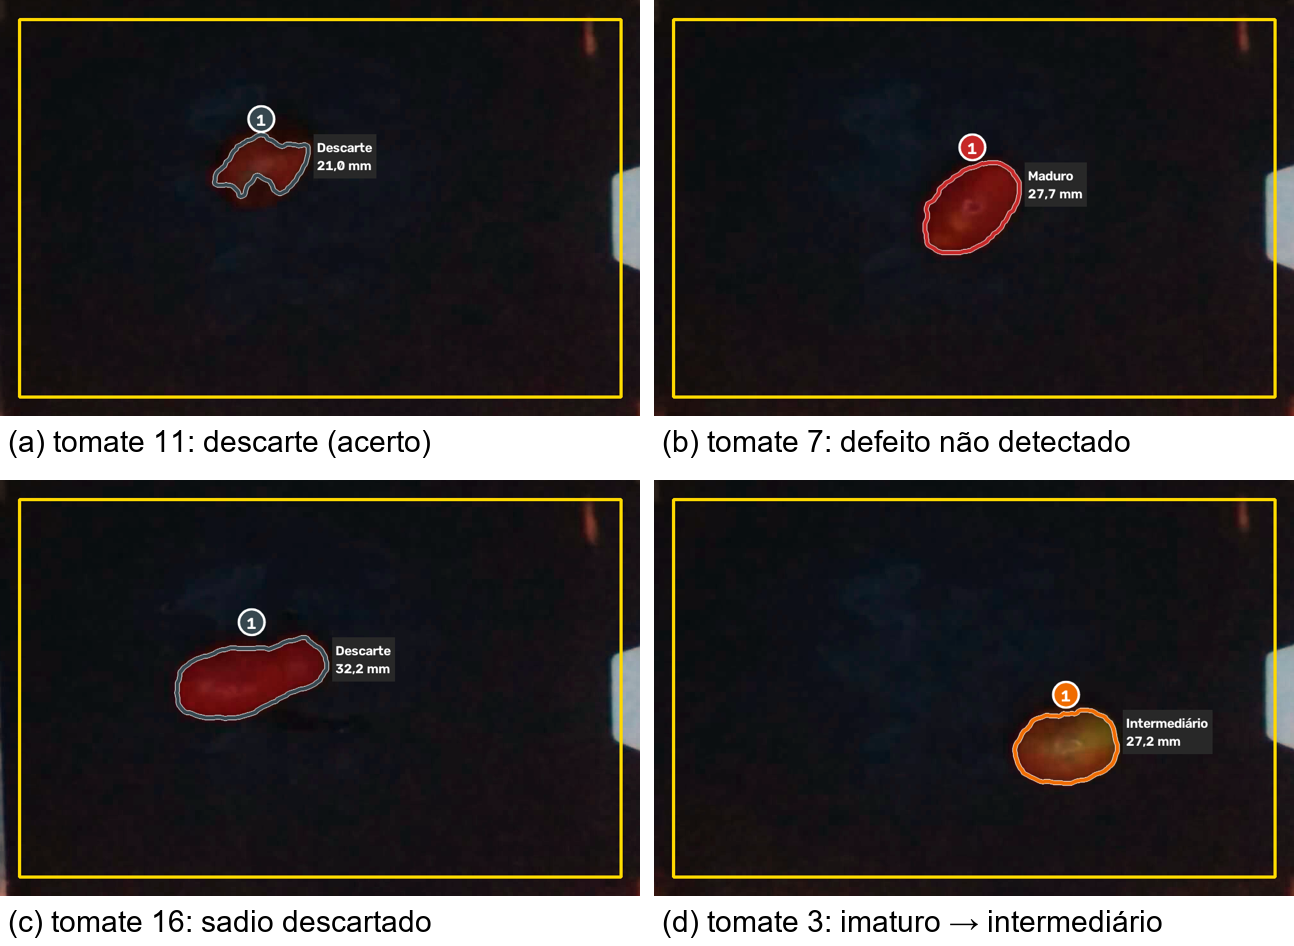
\includegraphics[width=\textwidth]{images/teste_exemplos.png}
	\fonte{Elaborado pelo autor (2026).}
\end{figure}

A acurácia balanceada no teste (86,8\%) ficou abaixo da média da validação cruzada (93,6\%), mas próxima da obtida nas sessões de captura intercaladas (cerca de 88,6\%). Três fatores contribuem para a diferença: o peso da primeira sessão na validação cruzada, discutido acima; a escolha da época de parada com os próprios dados de validação, que torna a validação cruzada otimista \cite{cawley2010}; e o tamanho do teste, em que um único erro muda a sensibilidade em 7,7 pontos percentuais e a especificidade em 11,1. O F1 de 0,88 atende ao critério de 0,85 na estimativa pontual, mas o intervalo de 0,71 a 1,00 e o limite inferior da sensibilidade (57,8\%) mostram que essa conclusão ainda é frágil.

% ----------------------------------------------------------
\section{Sistema Completo}
% ----------------------------------------------------------

Combinando a CNN e a LUT, o destino final foi correto em 18 dos 22 tomates do teste (81,8\%; IC 95\%: 61,5\% a 92,7\%). Dos quatro erros, dois são defeituosos que seriam enviados ao mercado como maduros (tomates 7 e 22), o erro de maior custo para o produtor; um é um tomate sadio descartado (tomate 16); e um é um imaturo enviado como intermediário (tomate 3). Os dois intermediários classificados como maduros pela LUT não afetaram o destino, porque ambos tinham defeito e foram corretamente descartados.

O tempo de processamento de uma imagem, do balanço de branco à decisão do destino, teve mediana de 53,5 ms (de 50,7 a 56,7 ms) no computador de desenvolvimento, com a CNN executada pelo OpenCV na CPU e as fotos lidas do disco, isto é, sem incluir a captura pela câmera. O valor está bem abaixo da meta de 200 ms por tomate e corresponde a cerca de 19 imagens por segundo.
% FIXME (autor): informar o processador e a memória do computador de desenvolvimento. A primeira inspeção, que inclui a carga do modelo, foi excluída dessa estatística. O tempo no computador da bancada não foi medido.

A IHM foi utilizada na bancada para classificar tomates com a câmera ao vivo, exibindo para cada fruto o destino, a maturação, a probabilidade de defeito e as medidas, e registrando as inspeções em CSV. Em um dos primeiros usos, com a versão preliminar da rede, um tomate verde e sem defeitos visíveis foi classificado como defeituoso. O conjunto de defeitos não tem rótulo de maturação, de modo que não é possível afirmar quantos tomates não vermelhos ele contém; esse caso ilustra a necessidade de que o treino cubra todas as variações de cor encontradas na operação.
% FIXME (autor): incluir uma captura de tela da IHM em operação.

% ----------------------------------------------------------
\section{Síntese e Limitações}
% ----------------------------------------------------------

O \autoref{qua:criterios} compara os resultados com os critérios de aceitação definidos no início do projeto.

\begin{quadro}[htb]
	\centering
	\caption{\label{qua:criterios}Resultados em relação aos critérios de aceitação.}
	\begin{tabular}{|p{3.3cm}|p{3.0cm}|p{4.6cm}|p{3.0cm}|}
		\hline
		\textbf{Requisito} & \textbf{Critério} & \textbf{Resultado} & \textbf{Situação} \\
		\hline
		Segmentação & $\geq$ 95\% das imagens & 22 de 22 (ou 21 de 22, se o tomate 16 for dois frutos) & Atendido \\
		\hline
		Calibração da escala & Erro $\leq$ 0,5 mm & Resíduo máximo de 0,46 mm no tabuleiro & Atendido \\
		\hline
		Diâmetro & Erro médio absoluto $\leq$ 1 mm & 0,45 mm com moeda; não validado em tomates & Parcial \\
		\hline
		Maturação (LUT) & Acurácia $\geq$ 90\% & 86,4\% (IC: 66,7\% a 95,3\%); 50\% de acerto médio por classe & Não atendido \\
		\hline
		Defeitos (CNN) & F1 $\geq$ 0,85 & F1 = 0,88 no teste (IC: 0,71 a 1,00) & Atendido (estimativa pontual) \\
		\hline
		Tempo de processamento & $\leq$ 200 ms por tomate & Mediana de 53,5 ms & Atendido \\
		\hline
	\end{tabular}
	\fonte{Elaborado pelo autor (2026).}
\end{quadro}

As principais limitações do estudo são:
\begin{alineas}
	\item \textbf{tamanho do conjunto de teste}: com 22 tomates, os intervalos de confiança têm largura de 29 a 42 pontos percentuais, e as classes imaturo e intermediário têm apenas 1 e 4 frutos;
	\item \textbf{iluminação}: a luz da bancada é fraca e fria, o que exigiu ganho de 2,33 no canal vermelho e produziu imagens escuras, com variação de 14,7\% do branco ao longo da região; isso afeta principalmente a LUT e a visibilidade de defeitos pequenos;
	\item \textbf{rótulos}: a maturação e os defeitos foram rotulados visualmente por uma única pessoa, sem medida de concordância entre avaliadores;
	\item \textbf{ordem de captura}: na primeira sessão, que domina o conjunto de defeitos, as classes foram fotografadas em sequência, e o desempenho da CNN foi menor nas sessões intercaladas;
	\item \textbf{independência do teste}: os tomates de teste são distintos dos de treino, mas foram fotografados na mesma madrugada que os últimos tomates de treino e provavelmente vêm da mesma compra;
	\item \textbf{amostras}: os tomates vieram de supermercado, e não de produtores;
	\item \textbf{medição}: o viés de $-0{,}45$ mm na escala não foi corrigido, a medida em tomates não foi comparada com paquímetro e o tamanho não é usado para separar os frutos em classes de calibre;
	\item \textbf{escopo}: o sistema classifica um tomate por imagem em uma bancada estática; a separação física por atuadores e a operação em esteira não foram implementadas.
\end{alineas}
